\section{Methods for prediction and analysis of roll damping}
\label{se:methods_for_prediction_and_analysis}
%\subsection{Equations}
%\label{se:equations}
From roll decay tests roll damping coefficients are normally derived based on the
logarithmic decrement of the roll peaks. However, this approach is sensitive to lowfrequency disturbances and noise, which does not have to be a problem in controlled
model test environment, but is difficult to avoid during full scale tests. An alternative
and more robust approach, which utilizes full time series of roll decay tests and
not only the peaks, is the numerical Parameter Identification Technique (PIT) as
described in IMO (2006) and also used in Bulian (2004). In this approach a numerical
solution to a one degree of freedom roll equation is fitted to the roll decay time series
by tuning the parameters in the roll equation.
To evaluate the performed tests, a modified version of the PIT approach is developed. This modified approach adds a time-dependent second-degree polynomial to
the fitting, that later can be separated from the solution to account for low frequency
disturbances. The roll equation that is used for the evaluation has a linear-quadratic
10 Assessment of Ship Roll Damping Through … 183
damping dependence and a linear restoring term. It should be noted that even though
the approach could well handle roll equations with higher order of non-linearities in
the damping term as well as a non-linear restoring term, the limited amplitudes at
which the roll decay tests was conducted cannot motivate advantages of higher order
models.
The equation of a freely oscillating roll motion with linear-quadratic damping can
in non-dimensional form be expressed as

The roll motion can be written as \cite{himeno_prediction_1981}:
\input{equations/roll_equation_himeno}

The equation express the roll moment [Nm] along a longitudinal axis though the centre of gravity.
Where $A_{44}$ is the virtual mass moment of inertia, $B_{44}$ is the roll damping moment and $C_{44}$ is the restoring moment. $M_{44}$ represents the external moment (usually moment from external waves).



\textbf{should one put the following descrption in the experimental description.}
The roll damping moment $B_{44}$ is the primary interest in this paper. The $B_{44}$ is determined using model scale roll decay tests. $B_{44}$ is determined using system identification, by finding the best fit to the following equation:
\begin{equation}
A_{44} \ddot{\phi} + \operatorname{B_{44}}\left(\dot{\phi}\right) + \operatorname{C_{44}}\left(\phi\right) = 0
\end{equation}

The external moment is zero during a roll decay test, since there are no external forces present.

The $B_{44}$ can be expressed as a series expansion:  
$ B_{44} = B_1\cdot\dot{\phi} + B_2\cdot\dot{\phi}\left|\dot{\phi}\right| + B_3\cdot\dot{\phi}^3 + ...$

Truncating this series at the cubic term gives a "cubic model":
\input{equations/roll_decay_equation_cubic}

Truncating this series at the quadratic term gives a "quadratic model":Truncating this series at the quadratic term gives a "quadratic model":
\begin{equation}
A_{44} \ddot{\phi} + \left(B_{1} + B_{2} \left|{\dot{\phi}}\right|\right) \dot{\phi} + \operatorname{C_{44}}\left(\phi\right) = 0
\end{equation}


Truncating this series at the linear term gives a "linear model":
\begin{equation}
A_{44} \ddot{\phi} + B_{1} \dot{\phi} + \operatorname{C_{44}}\left(\phi\right) = 0
\end{equation}


Peter Piehl \cite{henry_peter_piehl_ship_nodate} shows an analytical solution to the linear model in equation \ref{eq:roll_decay_equation_himeno_linear}, where the natural frequency of the motion is obtained by:
\begin{equation}
\omega_{0} = \sqrt{\frac{C}{A_{44}}}
\end{equation}


The roll damping and the natural frequency can be made non dimensional using the following expressions \cite{himeno_prediction_1981}: 
\input{equations/B44_hat_equation}
\begin{equation}
\omega_{hat} = \frac{\sqrt{2} \omega \sqrt{\frac{beam}{g}}}{2}
\end{equation}


%\subsection{Analytical solution}
\label{se:analytical_solution}
\input{2_methods_for_prediction_and_analysis/experimental_estimation}

\subsection{Existing semi-empirical methods}
\label{se:Existing semi-empirical methods}

The roll damping consists of linear and nonlinear components. At zero speed the nonlinear damping is caused by the two-dimensional separation at the bilge keel or near the bilge circle (Eddy damping $B_E$). While at speed the nonlinear damping is mainly caused by the hydrodynamic lift force on the hull, represented as lift damping $B_L$. $B_E$ vanishes at high speed ($F_n>0.15)$ \cite{ikeda_components_1978}.

The wave damping also changes at speed. Ikeda \cite{ikeda_components_1978} proposes a formula for the fraction between wave damping at speed and zero speed: $\frac{B_W}{B_{W0}}$

The Ikeda method has been used to calculate the roll damping for a PCTC vessel Faust \cite{soder_assessment_2019}.
\begin{figure}[h]
    \centering
    \includegraphics[width=\columnwidth]{figures/ikeda_faust.pdf}
    \caption{Roll damping components calculated with Ikeda method for PCTC Faust}
    \label{fig:ikeda_faust}
\end{figure}



The Ikeda method \cite{ikeda_roll_1978}, \cite{ikeda_eddy_1978}, \cite{ikeda_roll_1979}, \cite{ikeda_components_1978}, \cite{ikeda_velocity_1979} is the most well known semi empirical method to predict roll damping. 

\begin{equation} \label{eq:ikeda}
B = B_F + B_E + B_L + B_W + B_{BK}
\end{equation}

This method divides the roll damping into friction, eddy, lift, waves and bilge keel components (see equation \ref{eq:ikeda}. The wave and eddy components require strip method calculations. This is not an attractive option for the present study since that would require calculations with exact hull geometries to be carried out for all of the ships in the study. There exist however a \emph{Simplified Ikeda method} \cite{kawahara_simple_2011} that is instead used in this study to calculate the eddy component $B_E$ and wave component $B_W$. Figure \ref{fig:ikeda_vs_simplified} shows a comparison between roll damping components calculated with \emph{Ikeda} and \emph{Simplified Ikeda method}. The roll damping is under-predicted with the simplified method for this particular case which is expected according to the limitations of this method  \cite{kawahara_simple_2011}.

\begin{figure}[H]
    \centering
    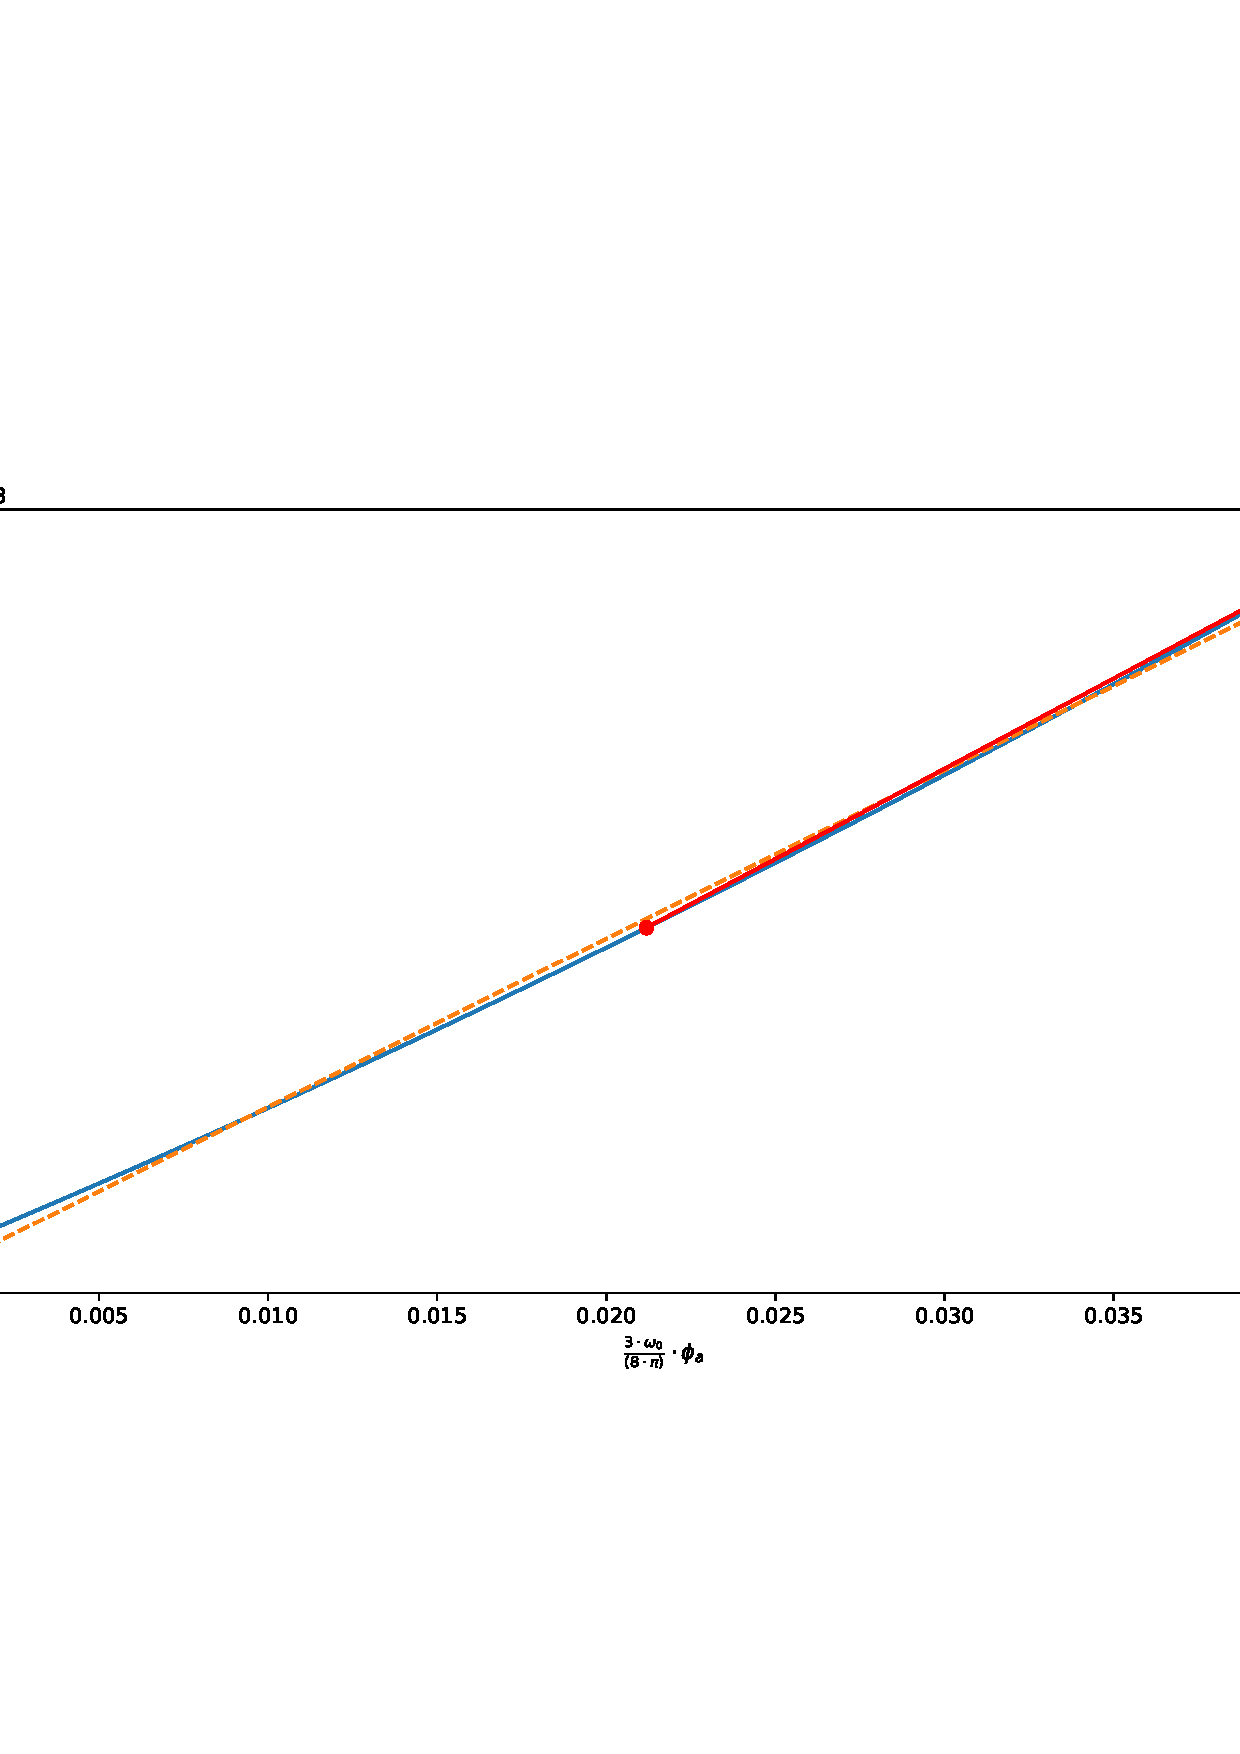
\includegraphics[width=\columnwidth]{figures/ikeda_B_1_B_2.pdf}
    \caption{Variation of roll amplitude to derive $B_1$ and $B_2$}
    \label{fig:ikeda_B_1_B2}
\end{figure}

A parameter variation was conducted in order to study the simplified method.
A "median ship" with the most usual parameters in the database was chosen as the baseline of the variation. The parameters were varied to the extreme values of the database, see figure \ref{fig:ship_parameters} for more details. 

Figure \ref{fig:ikeda_variation} shows this variation where all parameters have been none dimensionalized using froude scaling with $L_{pp}$ as scale factor. 
It seems that length to beam ratio between 0.23 and 0.24 has a huge peak. Also length to draft ratio below 0.034 has a large peak. 

\begin{figure}[H]
    \centering
    \includegraphics[width=0.9\columnwidth]{figures/ikeda_variation.pdf}
    \caption{Simplified method parameter variation}
    \label{fig:ikeda_variation}
\end{figure}


\section{Simplified Ikeda method}
\label{se:simplified_ikeda}
The \emph{Simplified Ikeda method} \cite{kawahara_simple_2011} has been implemented with the intention to be used both as a benchmark and maybe also as a sub-component of a new method. The examples from \cite{kawahara_simple_2011} was recalculated to check that the method has been implemented correctly.

Both  \emph{Simplified Ikeda method} can

The equivalent linear damping coefficient 
\begin{equation}
B_{e} = B_{1} + \frac{8 B_{2} \omega_{0} \phi_{a}}{3 \pi}
\end{equation}

